\section{Method}
\label{sec:method}
\begin{figure*}[t]
\centering
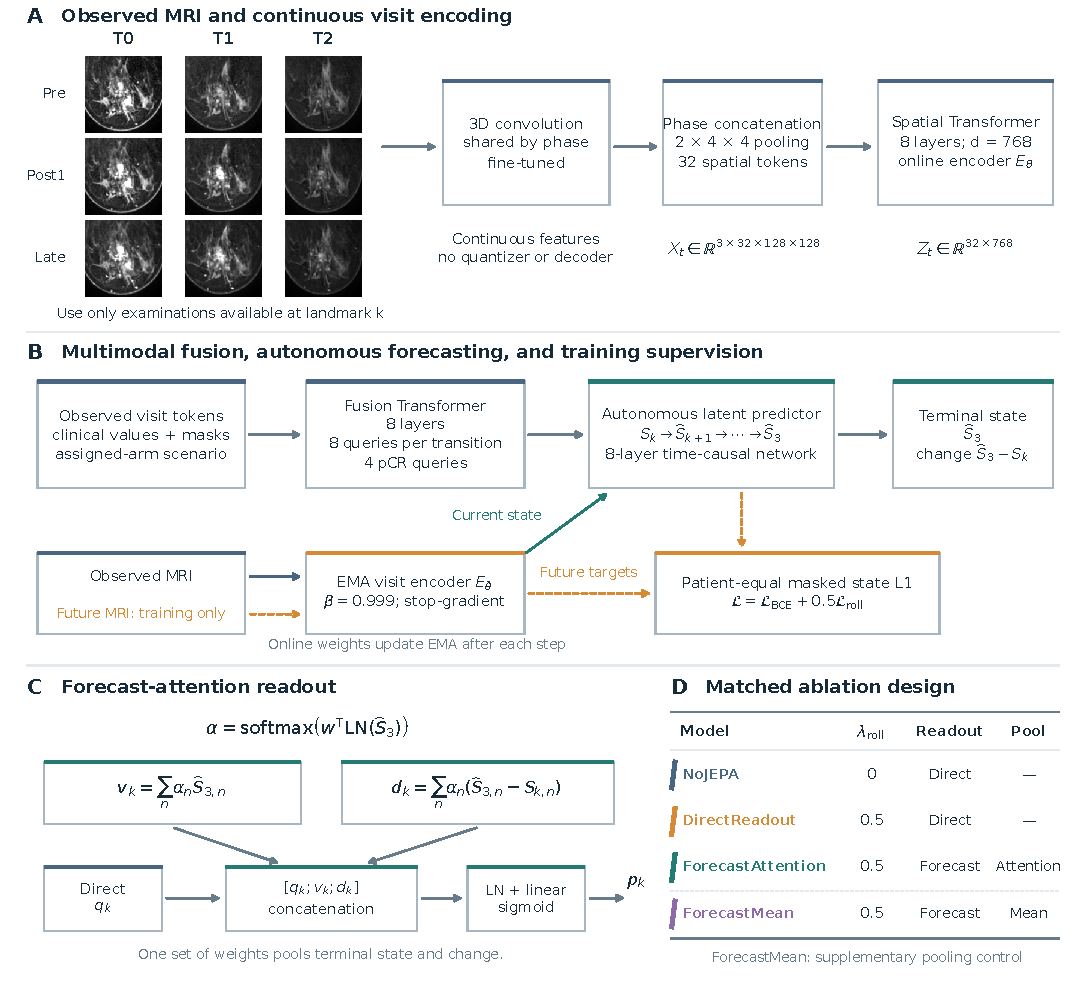
\includegraphics[width=\textwidth]{figures/framework.pdf}
\caption{Forecast-aware latent modeling and matched controls. (A) Real three-phase MRI crops from one development patient illustrate the same baseline-defined plane at T0, T1, and T2; the example and slice were selected without outcomes or model predictions. Only visits available at the prediction landmark are inputs. A shared continuous encoder and spatial Transformer produce visit tokens. (B) Clinical values, availability masks, and an assigned-arm scenario condition fusion and autonomous prediction to T3. The EMA encoder supplies the detached current state; available future MRI supplies training targets only. Dashed orange arrows denote training-target or loss paths. (C) Attention weights pool the predicted terminal state and its change; these features are combined with direct pCR-query features. (D) The primary variants separate removal of future-state supervision from the complete forecast readout. ForecastMean is a supplementary pooling control. MRI tiles are illustrative crops, not generated images, segmentation ground truth, or attention maps.}
\label{fig:framework}
\end{figure*}


\subsection{Longitudinal prediction problem}
\label{sec:problem}
We consider prediction of pathological complete response (pCR) from a patient's available magnetic resonance imaging (MRI) history during neoadjuvant treatment. Canonical examination stages are indexed by $t\in\{0,1,2,3\}$. At a prediction landmark $k\in\{0,1,2\}$, the model receives only examinations acquired and available by that landmark. Let $X_t\in\mathbb{R}^{3\times32\times128\times128}$ denote the processed examination at stage $t$, and let $o_t^{(k)}$ indicate whether this examination is available in the observed prefix. Missing examinations retain their canonical stage rather than shifting later examinations forward. The three channels contain the pre-contrast acquisition, the first post-contrast acquisition, and a metadata-selected late post-contrast acquisition, respectively. The late acquisition is not assumed to have the same acquisition index for all examinations.

The observed information is
\begin{equation}
 \mathcal{H}_k=\bigl\{(X_t,t):o_t^{(k)}=1\bigr\}\cup
 \bigl\{c_k,m_k,a_k,\tau_k\bigr\},
\end{equation}
where $c_k\in\mathbb{R}^{4}$ contains the available clinical variables, $m_k$ their availability indicators, $a_k$ the available assigned treatment-arm category, and $\tau_k$ its declared availability stage. The clinical variables are age at screening, hormone-receptor positivity, HER2 positivity, and a binary MammaPrint variable. Age is standardized using the current training partition; binary variables retain their original coding. Unavailable values are set to zero after standardization and accompanied by an explicit mask. The clinical token embeds the concatenated values and masks. Treatment conditioning uses 13 released arm categories and an additional unknown category. In this retrospective experiment, assigned arm and available baseline clinical variables are assumed to be known at T0. This is an assigned-arm scenario; the categorical input does not specify actual doses, treatment intervals, or treatment changes, and it does not support a causal interpretation.

The output is $p_k=\Pr(y=1\mid\mathcal{H}_k)$, where $y\in\{0,1\}$ is the final pCR label. Future MRI is stored separately as training supervision and is excluded from the prediction input. T3 can provide a future representation target during training, but is never a prediction landmark in the reported T0--T2 protocol.

\subsection{Continuous MRI encoding and multimodal fusion}
\label{sec:encoding}
Each observed examination is encoded independently by an online visit encoder $E_{\theta}$. Its convolutional front end shares the same single-channel weights across the three acquisition phases. Two stride-two three-dimensional convolutional stages, residual blocks, and group normalization produce 64 continuous feature channels per phase at one-quarter input resolution along each spatial axis. The three phase-specific feature maps are concatenated, adaptively averaged to a $2\times4\times4$ grid, and projected to a latent width of $d=768$. This gives $N=32$ spatial tokens per examination. Learned spatial positional embeddings and an eight-layer spatial Transformer then produce the visit representation $Z_t=E_{\theta}(X_t)\in\mathbb{R}^{N\times d}$.

The convolutional front end is initialized from the same pre-existing VQ-GAN-style codec checkpoint for all compared models and is fine-tuned. Here, the model uses continuous features from the codec encoder before its compression projection. It does not use discrete codebook assignments, a quantization objective, a decoder, or adversarial learning during downstream pCR training. \todo{Document the original codec pretraining dataset, patient-level overlap with the present partitions, checkpoint provenance, and applicable redistribution terms.}

Stage embeddings distinguish examination times. Observed image tokens, one clinical token, and one treatment-arm token form the multimodal context. An eight-layer fusion Transformer additionally receives eight learned transition-query tokens for each of the three canonical transitions and four pCR-query tokens. Transition-query slots are retained at every landmark, independently of which future targets happen to be available. Their conditioning is derived entirely from the observed prefix. Context tokens interact bidirectionally; appended transition and pCR queries use a causal attention mask and can attend to the context and preceding query positions. Padding masks remove unobserved image tokens. This produces transition features $A_{j+1}^{(k)}\in\mathbb{R}^{8\times d}$ for transitions $j\rightarrow j+1$, and pCR-query features $Q_k\in\mathbb{R}^{4\times d}$.

All spatial, fusion, and prediction Transformers use pre-normalization blocks, GELU feed-forward layers of width 3072, and dropout 0.3, following the attention-based architecture of \citet{vaswani2017}. Attention has 16 heads with 64 channels per head: its internal width is therefore 1024, followed by projection back to the 768-dimensional residual stream. The clinical and treatment tokens condition forecasting through the shared fusion network rather than through a separately supplied future treatment trajectory.

\subsection{EMA target states and autonomous forecasting}
\label{sec:forecasting}
A target visit encoder $E_{\bar\theta}$ is initialized as a copy of the online encoder and updated after each optimizer step by exponential moving average (EMA):
\begin{equation}
 \bar\theta\leftarrow\beta\bar\theta+(1-\beta)\theta,
 \qquad \beta=0.999.
\end{equation}
The target encoder remains in evaluation mode and receives no gradients. It defines a common representation space for the observed initial state and available future targets,
\begin{equation}
 S_t=\operatorname{stopgrad}\!\left(E_{\bar\theta}(X_t)\right)
 \in\mathbb{R}^{N\times d}.
\end{equation}
Encoding a future target in this branch supplies a loss target only; it does not make that examination available to the forecasting or classification input.

The predictor starts from the latest actually observed state in $\mathcal{H}_k$ and recursively advances to T3. For the reported landmarks, this initial state is $S_k$. At each future transition, it uses the corresponding transition features and its previously generated states. A history input additionally embeds the difference between a source state and its latest available predecessor, with a separate indicator for whether a predecessor exists. Observed history is used where available; after the landmark, the history is extended using model predictions. Thus, a missing future examination removes supervision at that time but does not interrupt the simulated transition sequence.

The prediction network is an eight-layer time-causal Transformer. Each transition block contains its eight transition tokens and 32 spatial source-state tokens, together with learned spatial and temporal embeddings. Tokens can interact within a block; attention between transition blocks is directed from earlier to later blocks. A learned root token remains available when some blocks are masked. The network predicts a residual state increment,
\begin{equation}
 \widehat S_{j+1}=\widetilde S_j+
 G_{\phi,j}\!\left(\widetilde S_{k:j},A_{k+1:j+1}^{(k)},D_{k:j}\right),
 \qquad j=k,\ldots,2,
\end{equation}
where $\widetilde S_k=S_k$, subsequent $\widetilde S_j$ are generated states, and $D_{k:j}$ denotes the available predecessor differences and validity indicators. The residual output projection is initialized to zero, so prediction initially preserves the source state. The transition features summarize the complete legal prefix even when only a subset of previous state differences is available to a particular prediction block.

Forecasts are generated autonomously during training and inference. A true future state never replaces a predicted predecessor. The classifier likewise uses this autonomous trajectory. The configuration includes no teacher-forced next-state loss in these experiments. EMA encoding of real future examinations is used exclusively to evaluate representation error against available targets.

\subsection{Prediction-conditioned pCR readout}
\label{sec:readout}
The full model, \fullmodel{}, combines a direct summary of the observed prefix with summaries of the predicted terminal state and its change from the current state. First, the four pCR-query features are averaged to obtain $q_k=\frac14\sum_{r=1}^{4}Q_{k,r}$. For spatial token $n$, the forecast change is $\Delta S_{k,n}=\widehat S_{3,n}-S_{k,n}$. A learned scalar scorer defines
\begin{equation}
 \alpha_{k,n}=
 \frac{\exp\!\left(w^{\mathsf T}\operatorname{LN}(\widehat S_{3,n})\right)}
 {\sum_{u=1}^{N}\exp\!\left(w^{\mathsf T}\operatorname{LN}(\widehat S_{3,u})\right)}.
\end{equation}
The same weights pool terminal state and change,
\begin{equation}
 v_k=\sum_{n=1}^{N}\alpha_{k,n}\widehat S_{3,n},
 \qquad
 d_k=\sum_{n=1}^{N}\alpha_{k,n}\Delta S_{k,n}.
\end{equation}
The final prediction is
\begin{equation}
 p_k=\sigma\!\left(b+u^{\mathsf T}
 \operatorname{LN}\!\left([q_k;v_k;d_k]\right)\right).
\end{equation}
The scorer is initialized with $w=0$, corresponding to uniform pooling at initialization. Classification gradients propagate through the generated terminal state, predictor, and transition-conditioning pathway. The observed EMA reference state remains detached. The attention weights summarize transformed spatial tokens and should not be interpreted as validated anatomical localization or tumor segmentation.

For \direct{}, pCR is instead predicted directly from $q_k$ using a layer-normalized linear head. Its future-state predictor is trained as an auxiliary task, but generated states are not explicit inputs to the pCR head. The direct head has input width $d$, whereas the full readout has width $3d$. Their comparison therefore evaluates the complete forecast-conditioned readout, including its state and change inputs and classifier width. An additional mean-pooling variant, when reported, retains the forecast-conditioned readout and replaces $\alpha_{k,n}$ by $1/N$.

\subsection{Training objective and matched ablations}
\label{sec:objective}
Let $\mathcal{B}_{y}$ be the labeled patients in a training batch, and let $m_{i,t}^{\mathrm{future}}$ indicate an actually available future target for patient $i$ after its sampled landmark. The pCR objective is unweighted binary cross-entropy,
\begin{equation}
 \mathcal{L}_{\mathrm{pCR}}=
 -\frac{1}{|\mathcal{B}_{y}|}\sum_{i\in\mathcal{B}_{y}}
 \left[y_i\log p_i+(1-y_i)\log(1-p_i)\right].
\end{equation}
Define $M_i=\sum_t m_{i,t}^{\mathrm{future}}$ and $\mathcal{B}_{+}=\{i:M_i>0\}$. Autonomous representation supervision is patient-equal:
\begin{equation}
 \mathcal{L}_{\mathrm{roll}}=
 \frac{1}{|\mathcal{B}_{+}|}\sum_{i\in\mathcal{B}_{+}}
 \frac{1}{M_i}\sum_t m_{i,t}^{\mathrm{future}}
 \frac{\|\widehat S_{i,t}-S_{i,t}\|_1}{Nd}.
\end{equation}
If a batch contains no future targets, this term is zero. Each available future examination has equal weight within a patient; the loss uses no horizon discount, lesion weighting, or fabricated target for a missing visit. Patients without future MRI still contribute pCR supervision.

The full model and \direct{} minimize
\begin{equation}
 \mathcal{L}=\mathcal{L}_{\mathrm{pCR}}+0.5\mathcal{L}_{\mathrm{roll}}.
\end{equation}
\nojepa{} uses the direct pCR head with $\mathcal{L}=\mathcal{L}_{\mathrm{pCR}}$. This historical control name denotes removal of future-state auxiliary supervision, rather than removal of every transition-related module: it retains the shared fusion architecture and transition-query slots. Consequently, \direct{} versus \nojepa{} isolates the added autonomous representation objective under the same direct readout, whereas \fullmodel{} versus \direct{} assesses the added forecast-conditioned classification pathway. The latter comparison cannot isolate spatial attention alone.

All three models omit teacher-forced JEPA, image reconstruction, flow-matching, and variance-regularization losses. In particular, the future objective reported here is autonomous state prediction, despite the JEPA-related implementation lineage. During training, patients are shuffled once per epoch and one actual available T0--T2 landmark is sampled uniformly for each patient. This balances patient contributions without treating a patient with more visits as several independently sampled patients. The same clinical endpoint supervises each sampled prefix; validation assesses all available eligible prefixes using patient-equal weighting.
